\documentclass[11pt,letterpaper]{article}
\usepackage[T1]{fontenc}
\usepackage{lmodern,amsmath,amssymb,amsthm,mathtools,booktabs,graphicx,xcolor,fancyhdr}
\usepackage[top=0.86in,bottom=0.85in,left=0.96in,right=0.96in,headheight=14pt,headsep=14pt]{geometry}
\usepackage{hyperref}
\definecolor{ink}{HTML}{183942}
\definecolor{accent}{HTML}{1D6667}
\hypersetup{colorlinks=true,linkcolor=accent,urlcolor=accent,citecolor=accent,pdftitle={Detecting nonreal zeros from sparse logarithmic derivatives},pdfauthor={OpenAI}}
\pagestyle{fancy}\fancyhf{}
\fancyhead[L]{\small\textcolor{accent}{Sparse logarithmic derivatives}}
\fancyhead[R]{\small\textcolor{accent}{Rational sampling centers}}
\fancyfoot[C]{\small\thepage}\renewcommand{\headrulewidth}{0.25pt}
\setlength{\parindent}{0pt}\setlength{\parskip}{4.4pt plus 1pt minus 1pt}
\setlength{\abovedisplayskip}{7pt plus 1pt minus 2pt}
\setlength{\belowdisplayskip}{7pt plus 1pt minus 2pt}
\raggedbottom
\newcommand{\Q}{\mathbb Q}\newcommand{\R}{\mathbb R}\newcommand{\C}{\mathbb C}
\newcommand{\Z}{\mathbb Z}\newcommand{\E}{\mathcal E}
\newcommand{\M}{\mathcal M}
\newcommand{\PSD}{\succeq 0}
\newcommand{\heading}[1]{\medskip\noindent{\large\bfseries\color{ink}#1}\par}
\newcommand{\thm}[2]{\noindent\textbf{\color{accent}#1.} \textit{#2}\par}
\begin{document}
\thispagestyle{plain}
{\small\bfseries\color{accent} ANALYTIC NUMBER THEORY \hfill 26 NOVEMBER 2026}\par
\vspace{0.16in}
{\fontsize{25}{29}\selectfont\bfseries\color{ink}Detecting nonreal zeros from\\ sparse logarithmic derivatives\par}
\vspace{4pt}
{\large Rational centers, powers of reciprocal zeros, and Hankel inertia\par}
\vspace{8pt}
\hrule height .6pt \vspace{5pt}

\textbf{Abstract.} Three fixed heights \(0,1,5\) detect a departure from the critical line for a completed Dirichlet \(L\)-function using logarithmic derivatives whose orders occupy a set of density zero. The stride can be chosen separately, and arbitrarily large, at each height. We prove a more general theorem for real entire functions of order at most one. We classify exactly the finite rational sets where the positivity test can fail, exhibit a quadratic attaining every exception, and determine the sharp total loss in counting distinct conjugate pairs across all rational centers. The proof combines a moving-window version of the Hermite moment argument with the cyclotomic cross-ratio restriction from discrete tomography.

\heading{1. What information is sampled?}
Let \(F\not\equiv0\) be entire of order at most one and real on \(\R\), up to a constant complex phase. At a real center \(c\), let \(r_c\) be its zero multiplicity and put \(F_c(z)=F(z)/(z-c)^{r_c}\), with the removable value filled in. Define, for \(k\ge2\),
\begin{equation}
 P_k(c)=-\frac{1}{(k-1)!}\left.\frac{d^k}{dz^k}\log F_c(z)\right|_{z=c}
       =\sum_{\gamma\ne c}(\gamma-c)^{-k}.                 \label{eq:power}
\end{equation}
Here and below zeros in sums carry their multiplicities. The local logarithm can be chosen arbitrarily. Hadamard factorization at \(c\) gives \eqref{eq:power} because each genus-one factor contributes \(-1/[k(\gamma-c)^k]\) to the logarithm's \(k\)-th Taylor coefficient. The exponential prefactor has linear logarithm. The sum converges absolutely since \(\sum_{\gamma\ne c}|\gamma-c|^{-2}<\infty\).

For a positive integer stride \(m\), an even \(K\ge2\), and width \(b\ge1\), form
\begin{equation}
 H(c,m;K,b)=\big[P_{m(K+i+j)}(c)\big]_{0\le i,j<b}.
 \label{eq:H}
\end{equation}
These real symmetric matrices use only \(2b-1\) derivative orders.

\thm{Theorem A}{Fix \(C=\{0,1,5\}\). At each \(c\in C\), choose any stride \(m_c\ge1\) and any sequences of even starts \(K_j\to\infty\) and widths \(b_j\to\infty\). Then all zeros of \(F\) are real if and only if every center has positive semidefinite matrices \eqref{eq:H} for all sufficiently large \(j\). If \(F\) has a nonreal zero, one fixed center has a negative eigenvalue for every sufficiently large \(j\).}

For example, \(K_j=2^j,\ b_j=j,\ j\ge1\), uses \(O((\log N)^2)\) derivative orders up to \(N\) at each center. Indeed \(m2^j\le N\) allows only \(O(\log N)\) blocks, with \(2j-1\) orders apiece. This counts specified derivatives of the logarithm. Computing them from ordinary Taylor coefficients of \(F\) can require lower orders too.

\newpage
\heading{2. What the negative eigenvalues count}
Fix \(c,m\). Map each zero different from \(c\) to \(u=(\gamma-c)^{-m}\). Combine equal values, adding their positive integer multiplicities \(a_u\). The set of distinct values is invariant under conjugation, is bounded, and has at most one accumulation point, \(0\). Write \(d_c\in\{0,1,\ldots,\infty\}\) for the number of distinct nonreal conjugate pairs among these values. For a real symmetric matrix \(H\), let \(\nu_-(H)\) count its strictly negative eigenvalues with multiplicity.

\thm{Theorem B (moving-window inertia)}{For every choice of \(K_j,b_j\) as in Theorem A,
\[
 \lim_{j\to\infty}\nu_-\!\left(H(c,m;K_j,b_j)\right)=d_c .
\]
A finite limit is attained at every sufficiently large index. When \(d_c=0\), every block is positive semidefinite from the start.}

\textit{Proof.}
Identify a real coefficient vector with \(p(t)=\sum_{i<b}x_i t^i\). Its quadratic form is
\begin{equation}
 Q_K(p)=\sum_u a_u u^K p(u)^2 .                           \label{eq:Q}
\end{equation}
The real nodes contribute nonnegative squares because \(K\) is even. At a conjugate pair the contribution is \(2a_u|u|^K\Re(e^{iK\arg u}p(u)^2)\). This has at most one negative direction. More explicitly, the single real linear condition \(\Im(e^{iK\arg(u)/2}p(u))=0\) makes that term nonnegative. Thus the negative index is at most \(d_c\) when \(d_c\) is finite.

For the reverse bound, choose \(s\) distinct nonreal pairs and a representative \(v_\ell\) of each in the upper half-plane. Set \(r=\min_\ell |v_\ell|>0\). Let \(A\) be the finite set of all distinct nodes with \(|u|\ge r\), and \(n=|A|\). The remaining nodes satisfy \(|u|\le q<r\) for some \(q>0\), since only finitely many nodes have modulus at least \(r/2\). If the remainder is empty its contribution is zero.

For each \(t\in\R^s\) interpolate a polynomial \(p=p_{K,t}\) of degree \(<n\) by assigning
\[
 p(v_\ell)=i e^{-iK\arg(v_\ell)/2}t_\ell,\qquad
 p(\bar v_\ell)=\overline{p(v_\ell)},\qquad
 p=0\quad\hbox{on all other nodes in }A .
\]
Uniqueness gives real coefficients. The Lagrange basis for \(A\) is fixed, so \(\sup_{|z|\le q}|p(z)|\le B\|t\|_2\) with \(B\) independent of \(K\). The contribution of \(A\) is \(-2\sum_\ell a_{v_\ell}|v_\ell|^K t_\ell^2\le-2r^K\|t\|_2^2\). The absolute contribution of the remaining nodes is at most
\[
 B^2\|t\|_2^2 q^{K-2}\sum_u a_u |u|^2 .
\]
The series is finite by \eqref{eq:power} and boundedness of the reciprocal nodes. As \(q/r<1\), the form is negative definite on this \(s\)-dimensional interpolation space for all large even \(K\), provided \(b\ge n\). Both requirements eventually hold. Taking \(s=d_c\) when finite and arbitrary \(s\) otherwise proves the claim. \hfill\(\square\)

The proof gives eventual detection along the prescribed blocks even when consecutive blocks use disjoint derivative orders. Exponentiation can identify different zeros or send a nonreal pair to a real value. The next two sections determine how much information this can conceal.

\newpage
\heading{3. Rational centers at which a pair is invisible}
For \(w=x+iy,\ y>0\), call \(c\in\R\) \emph{blind for \(w\) at stride \(m\)} if \((w-c)^{-m}\) is real. Consider the fractional linear map
\[
 T_w(t)=\frac{t-w}{t-\bar w},\qquad T_w(\infty)=1.
\]
It is injective on the real projective line and takes it onto the unit circle. Blindness is equivalent to \(T_w(c)^m=1\). In ordinary angle coordinates this reads
\begin{equation}
 c=x-y\cot(k\pi/m),\qquad 1\le k<m.                       \label{eq:cot}
\end{equation}
For several centers with different strides, their images and \(1\) all lie in a single group of roots of unity, by taking the least common multiple.

\thm{Cyclotomic lemma (Gardner--Gritzmann)}{If a cross ratio of four distinct roots of unity is rational and greater than one, it lies in
\[
 \E=\{4/3,\ 3/2,\ 2,\ 3,\ 4\}.
\]
If their orders divide \(m\), a prime \(p\nmid m\) divides neither the numerator nor the denominator of the reduced cross ratio or its complement.}

\textit{Proof of the restriction.} Write \(N\) for a common order and work in \(L=\Q(\zeta_N)\). For \(\xi\ne1\) of order \(d\mid N\), the absolute norm of \(1-\xi\) is \(\Phi_d(1)^{[L:\Q]/\varphi(d)}\). The identity \(\prod_{e\mid d}\Phi_e(X)=X^d-1\), with \(X-1\) removed and \(X=1\), gives \(\Phi_d(1)=p\) for \(d=p^a\) and \(1\) otherwise, by induction. Thus the normalized \(p\)-valuation of that norm (divide by \([L:\Q]\)) lies between 0 and \(1/(p-1)\), and vanishes for \(p\nmid N\).

For a difference of two roots the same bound holds, since their ratio is a root of unity and their individual norms are units. A cross ratio \(r\) and its complement \(1-r\) are each quotients of two products of two such differences. For rational \(r\) this proves
\[
 |v_p(r)|,\ |v_p(1-r)|\le 2/(p-1),
 \qquad v_p(r)=v_p(1-r)=0\ \text{if }p\nmid N .
\]
Write \(r=A/B>1\) in lowest terms and \(D=A-B\). The pairwise coprime positive integers \(A,B,D\) each divide \(12\). The possibilities for \(A=B+D\) are \(2=1+1,\ 3=1+2,\ 4=1+3\) and their reversals. These yield the list. This argument gives the restriction needed here. Gardner and Gritzmann also determine the root configurations in their Theorem 3.10 \cite{GG}. \hfill\(\square\)

For ordered rational centers \(a<b<c<d\) simultaneously blind for \(w\), invariance of cross ratios gives the following two necessary tests.
\begin{equation}
 \frac{c-a}{b-a}\in\E,\qquad
 \frac{(c-a)(d-b)}{(c-b)(d-a)}\in\E .                       \label{eq:ratios}
\end{equation}
The first uses \(\infty\) as the fourth point and a reordering. Both displayed expressions exceed one. In particular the triple \(0,1,5\) fails the first test. Any nonreal zero then has a nonreal image at one of those three centers, for any assigned strides. Theorem B proves Theorem A.

\newpage
\heading{4. Exact classification of all rational sampling sets}
Put \(\M=\{-3,-1,0,1,3\}\). An affine copy of \(\M\) is \(a+b\M\) with \(a,b\in\Q,\ b\ne0\).

\thm{Theorem C}{For a finite set \(C\subset\Q\), the following are equivalent.
\begin{enumerate}\setlength{\itemsep}{0pt}
\item Some nonreal \(w\) can be blind at every \(c\in C\), allowing any positive integer stride at each center.
\item \(C\) is contained in an affine copy of \(\M\).
\item A real quadratic polynomial with a nonreal pair passes every positivity test \eqref{eq:H} at every \(c\in C\), using the common stride \(6\).
\end{enumerate}}
Consequently six arbitrary distinct rational centers always suffice, and there are sets of five that fail. Three is the minimum number of \emph{chosen} centers uniformly sufficient for these tests with arbitrary strides.

\textit{Proof.} For \(|C|\ge2\), rescale its least and greatest elements to \(0,1\). By \eqref{eq:ratios}, each interior point is in \(X=\{1/4,1/3,1/2,2/3,3/4\}\). For a pair \(u<v\) in \(X\), applying \eqref{eq:ratios} to \(0,u,v,1\) leaves exactly
\[
 (1/4,1/2),\ (1/3,1/2),\ (1/3,2/3),\ (1/2,2/3),\ (1/2,3/4).
\]
This list follows by substitution in the ten possible pairs. For example \(1/4,3/4\) passes every triple test and fails the four-point test with value \(9/8\). Hence the interior is contained in one of
\[
 \{1/4,1/2\},\qquad \{1/3,1/2,2/3\},\qquad \{1/2,3/4\}.
\]
Including the endpoints, the maps \(4t-1,\ 6t-3,\ 4t-3\), respectively, put these three sets inside \(\M\). Singletons and the empty set satisfy the same containment.

Conversely \(w=i\sqrt3\) satisfies \eqref{eq:cot} at each point of \(\M\) for \(m=6\). If \(C\subset a+b\M\), the quadratic \((z-a)^2+3b^2\) realizes a nonreal pair blind at every center. Its folded nodes are real, so all even-start blocks are positive semidefinite. If the quadratic in (3) passes throughout, Theorem B ensures its pair is blind throughout, proving (1). Any two rational centers embed in an affine copy of \(\M\). \hfill\(\square\)

\begin{center}
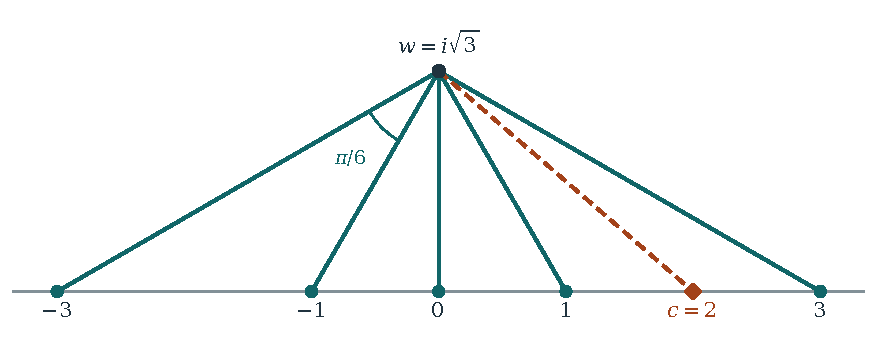
\includegraphics[width=0.85\linewidth,height=2.22in,keepaspectratio]{figures/rational_centers.pdf}\par
\end{center}
{\small\textbf{Figure 1.} Five rational centers see \(i\sqrt3\) along rays whose angles are multiples of \(\pi/6\). Adding the center \(2\) defeats every choice of strides, by Theorem C.}

\newpage
\heading{5. How many distinct pairs survive sampling?}
At a rational center \(c\) choose any integer \(m_c\ge1\) and let \(d_c\) be the limiting negative index in Theorem B. Each center may have its own starts and widths. Let \(D\) be the number of distinct nonreal conjugate pairs of zeros of \(F\).

\thm{Theorem D (total loss in the pair count)}{If \(D\) is finite, then
\begin{equation}
 0\le d_c\le D,\qquad
 \sum_{c\in\Q}(D-d_c)\ \le\ 5D+\binom D2.                 \label{eq:loss}
\end{equation}
Equality is attained for every \(D\) by an integer polynomial at common stride six. In particular \(d_c=D\) at all but finitely many rational centers. For \(D=\infty\), every sequence of distinct rational centers \(c_n\) satisfies \(d_{c_n}\to\infty\).}

\textit{Proof.} Represent each original pair by \(w_i=x_i+iy_i\) with \(y_i>0\). A pair incurs one unit of loss when its image is real. Each \(i\) does this at at most five rational centers by Theorem C, even with a different stride at each center. Among the remaining pairs, group together those with the same unordered image pair. A group of size \(h\) loses \(h-1\le\binom h2\) units. Real zeros always map to real values and play no part in these groups.

If two distinct pairs belong to the same group, the moduli of their images agree, so \(|w_i-c|=|w_j-c|\). For real \(c\) this is the equation
\begin{equation}
   2c(x_j-x_i)=|w_j|^2-|w_i|^2.                           \label{eq:bisector}
\end{equation}
It has at most one solution. If \(x_i=x_j\), distinct upper-half-plane representatives have unequal positive imaginary parts and the right side is nonzero. Summing first over original pairs and then over unordered pairs of pairs gives \eqref{eq:loss}.

For infinite \(D\), fix any \(s\) original pairs. Outside at most \(5s+\binom s2\) rational centers they yield \(s\) distinct nonreal image pairs by the same argument. Other zeros have positive multiplicities, so their presence cannot remove any of these images. This proves the infinite assertion. \hfill\(\square\)

\textbf{Attainment for every \(D\).} For \(j=0,\ldots,D-1\) put \(t_j=10\cdot2^j\), and at every center use stride six for
\[
 F_D(z)=\prod_{j=0}^{D-1}\bigl((z-t_j)^2+3\bigr).
\]
Pair \(j\) disappears at exactly \(t_j+\M\), by \eqref{eq:cot}. These \(5D\) centers are distinct. At \(c=(t_j+t_k)/2\), \(j<k\), the two upper roots minus \(c\) are negative conjugates, so their sixth reciprocal powers are conjugate. The midpoints are distinct by binary expansion. Each is divisible by \(5\) and equals no \(t_\ell\), since the sum of two distinct powers of two is not a power of two. It follows that no midpoint belongs to any \(t_\ell+\M\). Both images there are nonreal, and \eqref{eq:bisector} rules out any further simultaneous collision. Thus there are precisely \(5D\) disappearances and \(\binom D2\) two-pair mergers, all at different centers. This also proves the asserted sharpness when \(D=0\), with the empty product.

\newpage
\heading{6. Sampling centers that tolerate missing observations}
For a finite \(S\subset\Q\) with \(|S|\ge2\), write \(h(S)\) for its largest overlap with the five-point configuration, so that
\[
 h(S)=\max_{a,b\in\Q,\ b\ne0}|S\cap(a+b\M)|.
\]
The value is computable by matching any ordered pair of elements of \(\M\) to any ordered pair in \(S\) and testing the resulting five points.

\thm{Theorem E}{If \(F\) has any nonreal zero, at least \(|S|-h(S)\) centers in \(S\) have a negative eigenvalue in every sufficiently late block, for any choice of strides. The number \(|S|-h(S)\) is best possible for each \(S\).}

\textit{Proof.} Any particular nonreal pair is blind on a subset contained in an affine copy of \(\M\), by Theorem C. Theorem B detects it at all other centers. For equality choose \(a,b\) attaining the maximum and take \((z-a)^2+3b^2\) and stride six. By \eqref{eq:cot}, its rational blind centers are exactly \(a+b\M\). \hfill\(\square\)

\textbf{Dense integer designs.} For \(N\ge3\) one can choose \(N\) integer centers of diameter \(N\exp(O(\sqrt{\log N}))\) such that at least \(N-2\) centers detect any nonreal zero. This is the optimal number of detecting centers because any two specified rational centers can be simultaneously blind. In particular \emph{every three} centers from this design suffice, even if all other observations are lost.

To construct such sets, adapt Behrend's sphere argument \cite{Behrend}. A jointly blind triple \(A<C<B\) has \((C-A)/(B-A)\) in \(\{1/4,1/3,1/2,2/3,3/4\}\). Every forbidden equation therefore has the form
\[
       vC=(v-u)A+uB,\qquad 1\le u<v\le4 .
\]
Encode digit vectors from \(\{0,\ldots,M-1\}^k\) as integers in base \(4M\). A squared-norm level contains at least
\(M^k/(1+k(M-1)^2)\ge M^{k-2}/(k+1)\) vectors. On this level a forbidden equation holds digit by digit, since all coefficients on either side sum to at most four and each digit is less than \(M\). The digit vector for \(C\) would be a strict convex combination of two distinct vectors of the same norm, hence would have strictly smaller norm. This contradiction gives \(h(S)=2\) for any subset of the level with at least two elements.

Choose \(k=\lceil\sqrt{\log N}\rceil+3\) and \(M=\lceil((k+1)N)^{1/(k-2)}\rceil\), and take any \(N\) elements of a largest level. All encoded integers are less than \((4M)^k\), and
\[
 \log((4M)^k/N)\le k\log 8+
        \frac{2\log N+k\log(k+1)}{k-2}=O(\sqrt{\log N}).
\]
This use of Behrend's construction also connects to an internal method named in the upstream reading guide, which uses Behrend-type sparse sets to choose places of prescribed weight \cite{grh}.

\newpage
\heading{7. Prescribed strides and Dirichlet functions}

The cyclotomic proof gives a further distinction when \(m\) is prescribed. The table classifies sets \(C\) jointly blind for some nonreal point.
\begin{center}\small
\begin{tabular}{@{}ll@{}}\toprule
Common stride & Jointly blind finite rational sets\\ \midrule
\(m=1\) & Only the empty set\\
\(m=2\) & At most one center\\
odd \(m\ge3\) & At most two centers\\
even \(m\ge4,\ 3\nmid m\) & At most two, or a three-term arithmetic progression\\
\(6\mid m\) & Exactly the subsets of affine copies of \(\M\)\\ \bottomrule
\end{tabular}
\end{center}

To prove the table, observe that when \(m\) is odd, the numerator, denominator and their difference in any rational cross ratio would all be odd, an impossibility. When \(3\nmid m\), the three must all be prime to three, leaving only \(r=2\) in \(\E\). Thus any jointly blind triple in this case is an arithmetic progression, and four ordered numbers cannot have that property for all four triples. For \(m\ge3\) any two centers can be realized by choosing the two extreme cotangents in \eqref{eq:cot}, and scaling and translating them to the desired pair. For even \(m\ge4\), the middle cotangent is zero, realizing any progression. For \(6\mid m\) use the stride-six model. The cases \(m=1,2\) follow directly from \eqref{eq:cot}.

\textbf{A strip of known width.} Suppose all zeros satisfy \(|\Im z|<h\), \(h>0\). At common stride \(m\ge3\), two centers of separation \(\Delta\) always suffice for the class exactly when \(\Delta\ge 2h\cot(\pi/m)\). Indeed the extreme blind centers for \(x+iy\) in \eqref{eq:cot} are \(2|y|\cot(\pi/m)\) apart. Conversely, if \(\Delta\) is smaller, take \(x\) at the midpoint and \(y=\Delta/(2\cot(\pi/m))<h\). The conjugate pair \(x\pm iy\) gives a quadratic counterexample. This is sharp for the strip class of functions.

\textbf{Application to Dirichlet zeros.} Let \(\chi\) be primitive of conductor \(q>1\), and let \(a\in\{0,1\}\) satisfy \(\chi(-1)=(-1)^a\). Write
\[
 \Lambda(s,\chi)=(q/\pi)^{(s+a)/2}\Gamma((s+a)/2)L(s,\chi),\qquad
 F_\chi(z)=\epsilon_\chi^{-1/2}\Lambda(1/2+iz,\chi).
\]
Here \(\epsilon_\chi\) is the root number, with either square root of modulus one. The functional equation and conjugation give
\(\Lambda(s,\chi)=\epsilon_\chi\overline{\Lambda(1-\bar s,\chi)}\).
Thus \(F_\chi\) is real on the real axis, including for complex \(\chi\). Its order is one, and its zeros are the nontrivial zeros in ordinate coordinates \cite{Lfunctions}. A zero at \(s=\beta+it\) becomes \(\gamma=t+i(1/2-\beta)\). For the conductor-one character take \(F_1(z)=\xi(1/2+iz)\), where \(\xi(s)=s(s-1)\pi^{-s/2}\Gamma(s/2)\zeta(s)/2\). An imprimitive character has the same open-strip zeros as its primitive inducing character since the deleted Euler factors have zeros only on \(\Re s=0\).

Hence for each \(\chi\), critical-line reality is equivalent to Theorem A's three tests. Under Dirichlet GRH, \eqref{eq:Q} makes every finite block \emph{positive definite}. Indeed there are infinitely many distinct real zeros, each value of the power map has finite fibers, and a nonzero polynomial cannot vanish on all the real nodes.

\textbf{Two centers for \(\zeta\).} For a zero multiset also invariant under \(z\mapsto-z\), testing \(c\) also tests \(-c\). Corresponding matrix entries differ by \((-1)^{m(i+j)}\), a diagonal sign congruence. The two centers \(1,4\) therefore give the three effective centers \(-1,1,4\), whose ratio \(5/2\) is outside \(\E\). This applies to \(\xi\) and real primitive characters. A single fixed center cannot suffice uniformly over all strides in the class of even real entire functions. For \(c\ne0\), \(F(z)=z^2+c^2\tan^2(\pi/m)\) is blind at \(c\) for \(m\ge3\); at \(c=0\) use \(F(z)=z^2+1\) and \(m=2\).

\newpage
\heading{8. A worked example and comparison with the sources}
The rational quadratic \(F(z)=3z^2-3z+1\) has the conjugate roots
\[
 \gamma=\frac12+\frac{i}{2\sqrt3},\qquad \bar\gamma .
\]
They lie strictly inside the strip \(|\Im z|<1/2\) appropriate to Dirichlet ordinates. At stride six the two reciprocal powers both equal \(-27\) at each of \(c=0,1\). All blocks there are positive semidefinite of rank one. At \(c=5\) put \(u=(\gamma-5)^{-6}\). For \(K=2,\ b=2\) the determinant is
\[
 \det H = (u\bar u)^2(u-\bar u)^2
 = -\frac{11226235159675972800}{61^{24}}<0.
\]
The exact rational sign is a finite witness; the general theorem permits the first negative block to occur later. It does not give a precision guarantee for high-order numerical differentiation. The accompanying checker evaluates reciprocal powers and independently recovers the moments from the series for \(-F'/F\).

\textbf{The source connection.} In the pinned readable edition of \texttt{grh-lean}, \texttt{Statements.lean} fixes the five endpoints. \texttt{Main.lean} derives them from half-plane nonvanishing. The reading guide traces this back to the comparison of covolumes and a one-sided estimate for a twisted prime sum \cite{grh}. The Lean community's verification statement records the checks of Alp\"oge's original RH proof \cite{verification}. The Wikipedia article recalls the critical-line formulation and the distinction between trivial and nontrivial zeros \cite{wiki}. Its overview of Li's criterion and of Jensen polynomials gives two other ways in which positivity or real-rootedness encodes the critical-line statement.

ProveIt's inventory describes 61 research packets and says that placing them in the repository did not include independent checking or rebuilding. Its \emph{Torsion specialization and sparse prime sums} packet studies how a one-sided zero test survives restriction to a power grid of prime-sum arguments \cite{proveit}. The directory also has a later collection of 33 archives under \texttt{docs/incoming}. Two relevant examples are \texttt{grh\_zero\_certificates}, on contiguous Hermite matrices for finite zero windows, and \texttt{dirichlet\_li\_rigidity}, on stride ambiguities for Li coefficients. A third, \texttt{grh\_periods\_sampling\_and\_zeros}, uses consecutive logarithmic derivatives for a disk-centered census. The present paper asks when thinning derivative orders can conceal a nonreal zero. A targeted screen of all 33 archives is documented in \texttt{source\_screen.md}.

\textbf{Prior work and scope.} Hermite and Grommer moment criteria have a substantial history. Kytmanov and Khodos count nonreal zeros through full Hankel forms \cite{KK}. Bickel, Pascoe and Sargent study truncated positivity at real centers \cite{BPS}. Deng, Yang and L\"u treat coordinate images and finite contour moments \cite{DYL}. Gardner and Gritzmann's cyclotomic restriction \cite{GG} and the rational-angle classification of Dvornicich, Veneziano and Zannier \cite{DVZ} supply geometric precedents. The advances proposed here are the moving sparse blocks, their exact rational-center sampling rule, and the all-center loss estimate \eqref{eq:loss}. No identical combined result was located in the sources reviewed. Global publication priority is undetermined. The new results have mathematical proofs and exact finite checks. Our inspection of the upstream Lean project was at source level.

\textbf{Further research questions.} At a prescribed odd stride, when can the separate bounds for disappearances and collisions be attained together? Under explicit separation assumptions on a bounded set of zeros, how much absolute precision on each \(P_k(c)\) suffices to certify a negative eigenvalue? Finally, how does the exceptional-set classification change for centers in a fixed real quadratic field?

\newpage
\heading{References and source revisions}
\begingroup\small
\renewcommand{\refname}{}
\vspace{-2.0em}
\begin{thebibliography}{10}
\setlength{\itemsep}{5pt}
\bibitem{grh} L. Sernau and collaborators, \emph{GRH for Dirichlet \(L\)-functions, in Lean 4}, readable edition. Revision
\texttt{72fead102f663d5c7a407964a13dc0cf9d977207}.
\href{https://github.com/lsernau/grh-lean/blob/72fead102f663d5c7a407964a13dc0cf9d977207/grh/GUIDE.md}{Reading guide},
\href{https://github.com/lsernau/grh-lean/blob/72fead102f663d5c7a407964a13dc0cf9d977207/grh/src/Statements.lean}{statements} and
\href{https://github.com/lsernau/grh-lean/blob/72fead102f663d5c7a407964a13dc0cf9d977207/grh/src/Main.lean}{main proofs}.
\bibitem{verification} Lean FRO and Mathlib Initiative, \emph{Lean verification of the Riemann Hypothesis}, 21 November 2026.
\href{https://leanprover-community.github.io/blog/posts/riemann-hypothesis/}{Joint statement}.
The \href{https://github.com/leanprover-community/riemann-hypothesis}{community repository} also records the Dirichlet endpoints and the transition to the shorter edition.
\bibitem{proveit} V. Reshetnikov, \emph{ProveIt}, revision
\texttt{a9ae674322c8c4cce1bb2262e577733d3959d741}.
\href{https://github.com/VladimirReshetnikov/ProveIt/tree/a9ae674322c8c4cce1bb2262e577733d3959d741/Analysis/GeneralizedRiemannHypothesis}{GRH research inventory}.
See also the \href{https://github.com/VladimirReshetnikov/ProveIt/tree/a9ae674322c8c4cce1bb2262e577733d3959d741/Analysis/GeneralizedRiemannHypothesis/Research/grh-torsion-and-prime-sampling}{sparse prime-sampling packet}.
\bibitem{wiki} Wikipedia, \emph{Riemann hypothesis}, consulted 26 November 2026.
\href{https://en.wikipedia.org/wiki/Riemann_hypothesis}{Article}.
\bibitem{Lfunctions} NIST Digital Library of Mathematical Functions,
\href{https://dlmf.nist.gov/25.15}{\S25.15, Dirichlet \(L\)-functions}.
See also H. Davenport, \emph{Multiplicative Number Theory}, 3rd ed., Springer, 2000, chs. 9 and 16.
\bibitem{Behrend} F. A. Behrend, \emph{On sets of integers which contain no three terms in arithmetical progression}, Proc. Natl. Acad. Sci. USA \textbf{32} (1946), 331--332.
\href{https://doi.org/10.1073/pnas.32.12.331}{DOI}.
\bibitem{GG} R. J. Gardner and P. Gritzmann, \emph{Discrete tomography: determination of finite sets by X-rays}, Trans. Amer. Math. Soc. \textbf{349} (1997), 2271--2295, especially Theorem 3.10.
\href{https://doi.org/10.1090/S0002-9947-97-01741-8}{DOI}.
\bibitem{DVZ} R. Dvornicich, F. Veneziano and U. Zannier, \emph{Classification of rational angles in plane lattices}, Bull. Amer. Math. Soc. \textbf{59} (2022), 191--226.
\href{https://doi.org/10.1090/bull/1723}{DOI}.
\bibitem{KK} A. M. Kytmanov and O. V. Khodos, \emph{On localization of zeros of an entire function of finite order of growth}, Complex Anal. Oper. Theory \textbf{11} (2017), 393--416.
\href{https://doi.org/10.1007/s11785-016-0606-8}{DOI}.
\bibitem{BPS} K. Bickel, J. E. Pascoe and M. Sargent, \emph{Zero-free regions near a line}, Math. Z. (2023).
\href{https://doi.org/10.1007/s00209-023-03364-w}{DOI}.
\bibitem{DYL} Z. Deng, X. Yang and H. L\"u, \emph{Contour Hankel dynamics and indicator fields for the Riemann \(\Xi\)-function}, preprint (2026).
\href{https://arxiv.org/abs/2608.11520}{arXiv:2608.11520}.
\end{thebibliography}
\endgroup
\end{document}

